\chapter{利用插入代码实现VxWorks文件操作监控}

\section{目标与背景}

\subsection{目标}

本节中,我们利用前文
提供的代码插入和劫持函数的方法,
尝试在VxWorks镜像文件中,
插入一段代码并劫持dosFs文件系统的函数。
从而当系统中的应用程序进行文件读写操作时,
可以截获这一操作,
并在屏幕上打印操作的内容和相关信息。

\subsection{dosFs文件系统}

VxWorks文件系统中的dosFs是MS-DOS兼容的文件系统,
可基于块对物理介质进行操作。
它提供极大的灵活性以满足实时应用的各种要求。
在VxWorks操作系统中,
文件系统的位置位于IO系统和驱动程序之间。
它们之间的层次结构如图\ref{iosys}所示。

\begin{figure}[h!]
    \centering
    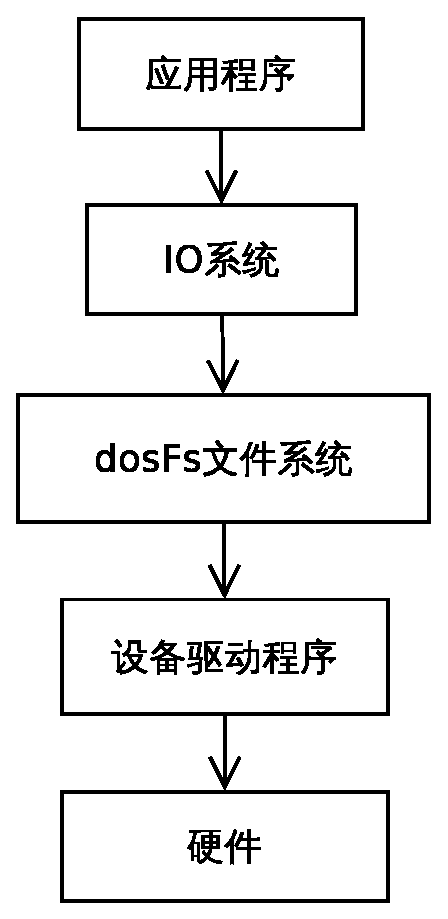
\includegraphics[width=0.21\textwidth]{figure/IOsys.eps}
    \caption{VxWorks中的IO系统图示}
    \label{iosys}
\end{figure}

具体到某个文件操作,例如open操作。
应用程序可以调用
库函数或者直接使用IO函数的时候,
他们都会调用dosFs中的dosFsOpen函数,
进而再调用驱动程序对应的函数。
最后达到访问硬件的目的。整个流程如图\ref{open}

\begin{figure}[h!]
    \centering
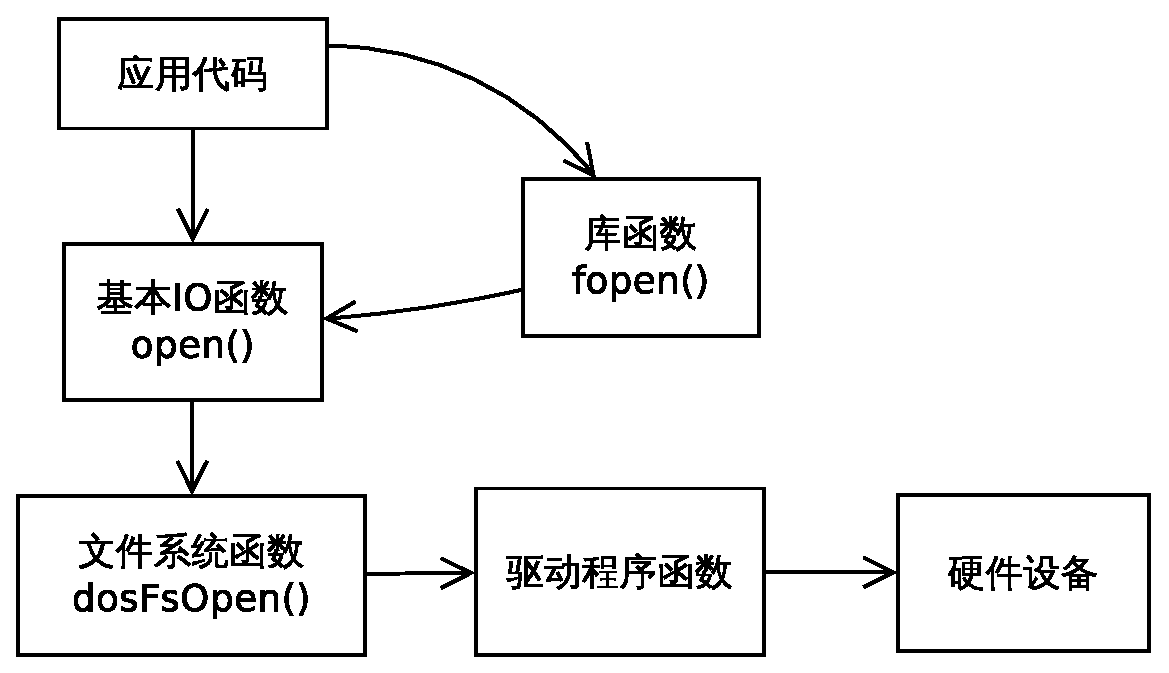
\includegraphics[width=0.55\textwidth]{figure/open.eps}
    \caption{打开一个文件的函数调用流程}
    \label{open}
\end{figure}

\section{劫持过程介绍}

\subsection{劫持位置的选择}

我们以劫持打开文件操作为例,
阐述进行文件操作劫持的原理。
首先我们要考察劫持的位置,
即在图\ref{open}所示的哪一层的相应函数中插入跳转,
执行我们的插入代码。
我们选择对文件系统函数进行劫持,即dosFsOpen()。
因为无论上层代码使用何种方式来进行文件操作,
即无论使用哪一个库,
都会最终调用到dosFsOpen(),
dosFsOpen()函数的原型如代码\ref{open_prototype}所示。

%% open函数的原型,C代码

\begin{lstlisting}[
  language={C},
  caption={dosFsOpen()函数原型},
  label={open_prototype},
]
LOCAL DOS_FILE_DESC_ID dosFsOpen
    (
    DOS_VOLUME_DESC_ID  pVolDesc, /* pointer to volume descriptor */
    char *      pPath,  /* dosFs full path/filename */
    int         flags,  /* file open flags */
    int         mode    /* file open permissions (mode) */
    );
\end{lstlisting}

可见,dosFsOpen函数的
传入参数包含了
文件路径、文件打开的权限等信息。
这也就意味着我们可以利用插入代码获取这些信息。
而如果在更低层的驱动层来进行劫持,
文件路径等信息就消失了,
劫持工作很大程度上失去了意义。

\subsection{劫持函数跳转流程}

为了不影响dosFsOpen的正常运行。
插入代码需要保证不污染原先的堆栈和寄存器。
为了在编写插入代码时不考虑这些问题,
而是当作编写一个正常的函数来进行,
我们继续使用“中间层”的思路。
我们称这一中间层为“proxy”,
控制流首先从dosFsOpen转移到proxy。
用于劫持的功能的代码则被分离出来,
单独写为一个函数,叫做hookFsOpen()。
图\ref{proxy}展示了劫持dosFsOpen函数的跳转过程。

\begin{figure}[h!]
    \centering
    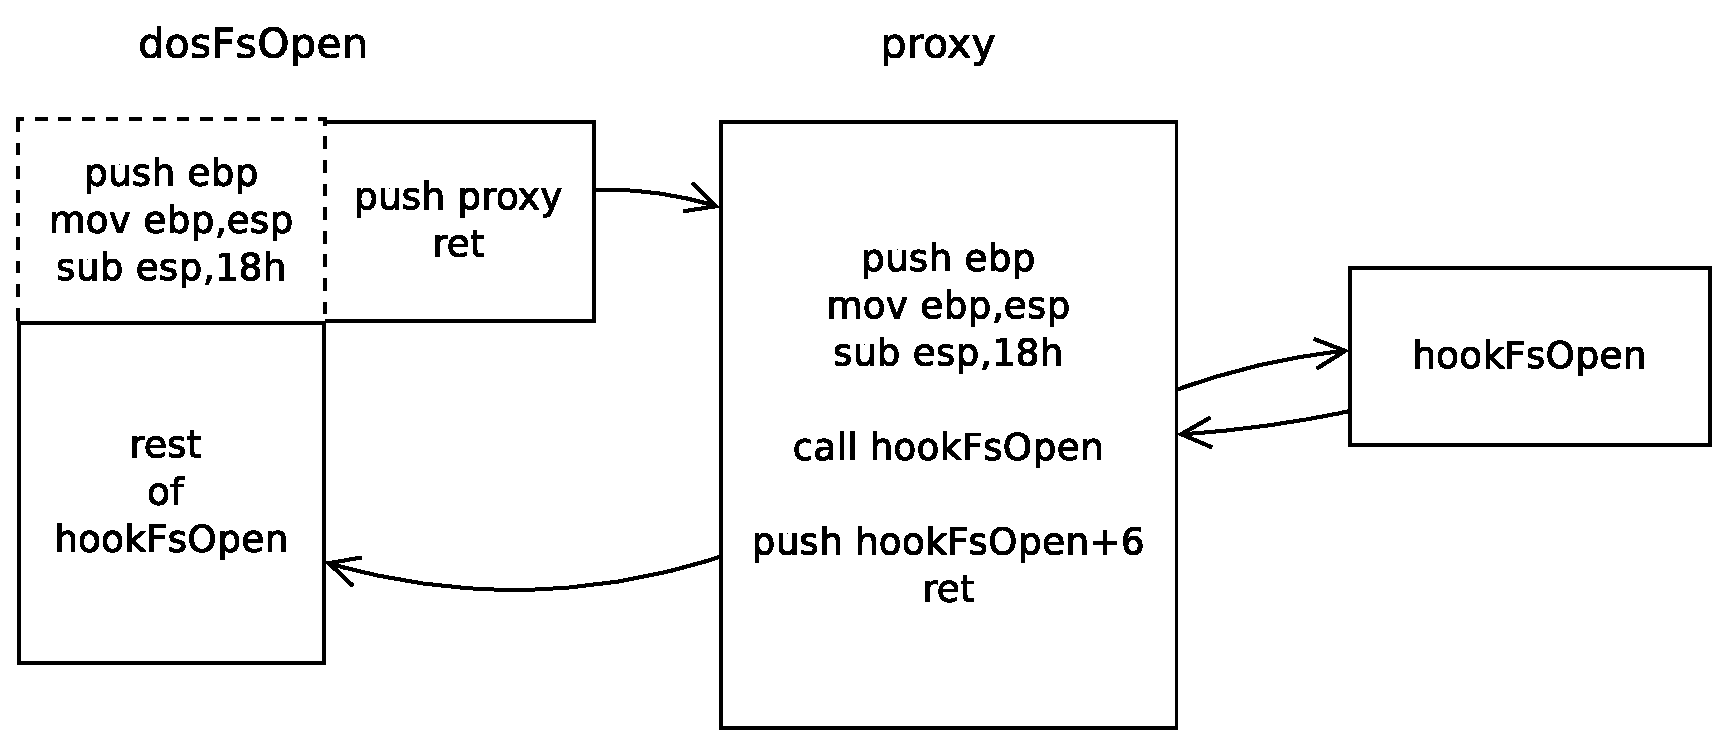
\includegraphics[width=0.76\textwidth]{figure/proxy.eps}
    \caption{劫持dosFsOpen的函数跳转流程}
    \label{proxy}
\end{figure}

我们将dosFsOpen函数开头的三条指令(位于虚线框中)替换为
右边方框的指令。
并在proxy开头补充这三条指令。
这样一来,proxy就很自然地拓展了dosFsOpen函数的空间,
可以在其中写入任何代码,
只需要在最后返回即可。
我们在proxy中使用call指令调用hookFsOpen函数,
一方面避免了在proxy中进行堆栈和寄存器的恢复;
另一方面,
我们hook函数不必真的像“插入”的函数那样小心翼翼,
担心污染了寄存器和堆栈。
总之,我们可以像编写正常的C语言函数一样,
来编写hookFsOpen()。

\subsection{劫持函数的插入}

假设我们已经写好了hookFsOpen.c,

为了能够一次性完成proxy和劫持函数的插入,
我们将hookFsOpen.c编译为汇编代码,
并在汇编代码中写入proxy代码,
利用汇编代码的标签功能,
proxy可以通过相对寻址找到hookFsOpen的位置。
汇编代码形如代码\ref{finish}所示。
\begin{lstlisting}[
 language={[x86masm]Assembler},
 caption={为插入而准备的汇编代码},
 label={finish},
]
global _start
section .text
_start:
    push ebp
    mov ebp,esp
    sub esp, 0x18            ; 补上dosFsOpen开头被替换的指令
    call hookFsOpen          ; 调用hookFsOpen,可通过相对寻址定位
    push dosFsOpen+6
    ret                      ; 返回至dosFsOpen第四条指令处

hookFsOpen:
    ......
    ......                   ; hookFsOpen函数体
\end{lstlisting}

接下来,
即可利用前文介绍的任何一种可行的方法,
将代码\ref{finish}进行汇编后,
插入VxWorks系统镜像的合适位置。
插入完成后,我们还需要进行几项修补和重定位工作:

1、修改dosFsOpen函数的开头三条指令,跳转至proxy开始处。

2、填写proxy中返回dosFsOpen()函数第四条指令的地址。

3、对于hookFsOpen()中所有的函数引用(例如printf),修正其绝对地址。

至此,我们完成了对open一个文件的操作的劫持。


\section{劫持函数的实现与测试}

为了完整地实现对文件操作进行监控,
我们完善了针对6项基本文件操作(create,delete,open,close,read和write)的劫持函数,
见附录\ref{hook}。
其中大量使用了gcc的内嵌汇编功能,
目的是通过读取栈来获得dosFs函数的参数。
劫持函数主要实现了两个功能:

1、获取和解析dosFs函数的参数;

2、调用printf打印操作名称,文件路径(pPath参数)和系统时间。

本节我们在完成对这四项文件操作
进行劫持的基础上,
编写测试用例进行测试。测试用例代码见代码\ref{file}。

\begin{lstlisting}[
  language={C},
  caption={operate\_file()函数源代码},
  label={file},
]
void operate_file(){
     int fd; 
     int nWritten,nRead;
     char read_buf[20]; 
     char *write_buf = "Hello dosFs!!!";

     memset(read_buf,0,sizeof(read_buf));
     fd = open("/DOSB/test1", O_CREAT | O_WRONLY, 0644);

     nWritten = write(fd, write_buf, 15);
     close(fd);
     fd = open("/DOSB/test1", O_CREAT | O_RDONLY, 0644);
     nRead = read(fd, read_buf, 20);

     printf("fd:%d,write:%d,read:%d,contains:%s\n",fd, nWritten,nRead,read_buf);
}
\end{lstlisting}


在一个文件系统被劫持的VxWorks中,
运行这一函数的结果如图\ref{after}所示。

\begin{figure}[h!]
    \centering
    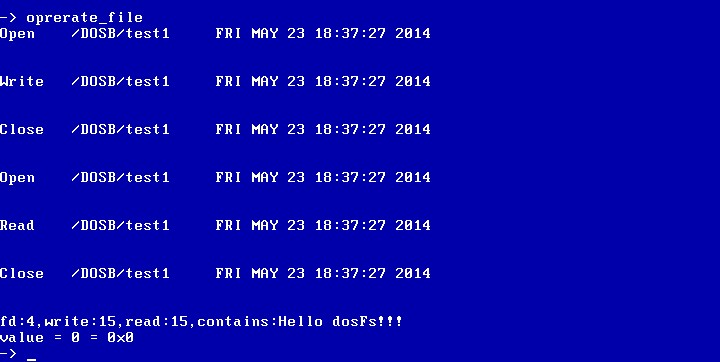
\includegraphics[width=0.55\textwidth]{figure/after.jpg}
    \caption{测试程序运行结果}
    \label{after}
\end{figure}

从该函数的输出中可以看出,
测试用例中每次调用文件操纵函数,
屏幕中都会打印一行输出,
输出的信息包含三个部分,
分别是操作的内容,目标文件路径和系统时间。
至此,我们已经达到了对使用dosFs文件系统的
VxWorks系统中的文件操作函数进行监控的目标。











